\documentclass[sigconf]{acmart}

%%
%% \BibTeX command to typeset BibTeX logo in the docs
\AtBeginDocument{%
  \providecommand\BibTeX{{%
    \normalfont B\kern-0.5em{\scshape i\kern-0.25em b}\kern-0.8em\TeX}}}

%% Rights management information.  This information is sent to you
%% when you complete the rights form.  These commands have SAMPLE
%% values in them; it is your responsibility as an author to replace
%% the commands and values with those provided to you when you
%% complete the rights form.
\setcopyright{acmcopyright}
\copyrightyear{2023}
\acmYear{2023}
\acmDOI{XXXXXXX.XXXXXXX}

%% These commands are for a PROCEEDINGS abstract or paper.
\acmConference[Conference acronym 'XX]{Make sure to enter the correct
  conference title from your rights confirmation emai}{June 03--05,
  2018}{Woodstock, NY}
\acmPrice{15.00}
\acmISBN{978-1-4503-XXXX-X/18/06}


%%
%% Submission ID.
%% Use this when submitting an article to a sponsored event. You'll
%% receive a unique submission ID from the organizers
%% of the event, and this ID should be used as the parameter to this command.
%%\acmSubmissionID{123-A56-BU3}

%%
%% For managing citations, it is recommended to use bibliography
%% files in BibTeX format.
%%
%% You can then either use BibTeX with the ACM-Reference-Format style,
%% or BibLaTeX with the acmnumeric or acmauthoryear sytles, that include
%% support for advanced citation of software artefact from the
%% biblatex-software package, also separately available on CTAN.
%%
%% Look at the sample-*-biblatex.tex files for templates showcasing
%% the biblatex styles.
%%

%%
%% The majority of ACM publications use numbered citations and
%% references.  The command \citestyle{authoryear} switches to the
%% "author year" style.
%%
%% If you are preparing content for an event
%% sponsored by ACM SIGGRAPH, you must use the "author year" style of
%% citations and references.
%% Uncommenting
%% the next command will enable that style.
%%\citestyle{acmauthoryear}

%%
%% end of the preamble, start of the body of the document source.
\begin{document}

%%
%% The "title" command has an optional parameter,
%% allowing the author to define a "short title" to be used in page headers.
\title{Dependability Analysis - Apache commons-imaging library}

%%
%% The "author" command and its associated commands are used to define
%% the authors and their affiliations.
%% Of note is the shared affiliation of the first two authors, and the
%% "authornote" and "authornotemark" commands
%% used to denote shared contribution to the research.
\author{Julian Alexis Orcinoli}
\authornote{All authors contributed equally to this research.}
\affiliation{%
  \institution{Università degli Studi di Salerno}
  \city{Fisciano}
  \state{Salerno}
  \country{Italy}
  \postcode{84084}
}
\email{j.orcinoli@studenti.unisa.it}

\author{Santiago Morales Henao}
\authornote{All authors contributed equally to this research.}
\affiliation{%
  \institution{Università degli Studi di Salerno}
  \city{Fisciano}
  \state{Salerno}
  \country{Italy}
  \postcode{84084}
}
\email{s.moraleshenao@studenti.unisa.it}

\author{Franco Nicolás Merenda}
\authornote{All authors contributed equally to this research.}
\affiliation{%
  \institution{Università degli Studi di Salerno}
  \city{Fisciano}
  \state{Salerno}
  \country{Italy}
  \postcode{84084}
}
\email{f.merenda2@studenti.unisa.it}


%%
%% By default, the full list of authors will be used in the page
%% headers. Often, this list is too long, and will overlap
%% other information printed in the page headers. This command allows
%% the author to define a more concise list
%% of authors' names for this purpose.
\renewcommand{\shortauthors}{Julian A. Orcinoli, Merenda F. Nicolas, and Santiago M. Henao}

%%
%% The abstract is a short summary of the work to be presented in the
%% article.
\begin{abstract}
  This paper presents a comprehensive analysis of software dependability in the context of the Apache Commons Imaging project, a vital component of the Apache Commons IO ecosystem. The study employs a multifaceted approach, leveraging software analytics, testing tools, and vulnerability assessment techniques to evaluate and enhance the dependability and code quality of the project.

  The analysis begins with an exploration of SonarCloud, delving into the identification and resolution of bugs. Subsequently, various software testing tools, including JaCoCo, CodeCov, PiTest, EvoSuite, and Randoop, are employed to assess code coverage, mutation testing, and automated test case generation. The study extends to vulnerability checking using OWASP Dependability Checker and FindSecBugs.
  
  Results showcase improvements in code quality, increased code coverage, and the identification and remediation of software vulnerabilities. The paper contributes valuable insights into the efficacy of diverse tools and methodologies in ensuring software dependability. Through this investigation, we aim to provide a nuanced understanding of the strengths and limitations of each approach, offering guidance for future endeavors in the pursuit of reliable and robust software systems.
\end{abstract}

%%
%% The code below is generated by the tool at http://dl.acm.org/ccs.cfm.
%% Please copy and paste the code instead of the example below.
%%
\begin{CCSXML}
<ccs2012>
   <concept>
       <concept_id>10011007.10011074.10011099.10011102.10011103</concept_id>
       <concept_desc>Software and its engineering~Software testing and debugging</concept_desc>
       <concept_significance>500</concept_significance>
    </concept>
    <concept>
       <concept_id>10011007.10011006.10011073</concept_id>
       <concept_desc>Software and its engineering~Software maintenance tools</concept_desc>
       <concept_significance>500</concept_significance>
   </concept>
   <concept>
       <concept_id>10011007.10011074.10011134.10003559</concept_id>
       <concept_desc>Software and its engineering~Open source model</concept_desc>
       <concept_significance>300</concept_significance>
   </concept>

 </ccs2012>
\end{CCSXML}

\ccsdesc[500]{Software and its engineering~Software testing and debugging}
\ccsdesc[500]{Software and its engineering~Software maintenance tools}
\ccsdesc[300]{Software and its engineering~Open source model}


%%
%% Keywords. The author(s) should pick words that accurately describe
%% the work being presented. Separate the keywords with commas.
\keywords{Software Dependability, Apache Commons Imaging, Software Analytics, SonarCloud, Software Testing Tools, Code Coverage, JaCoCo, CodeCov, Mutation Testing, PiTest, Java Microbenchmark Harness, JMH,  Automated Test Case Generation, EvoSuite, Randoop, Software Vulnerabilities, OWASP Dependability Checker, FindSecBugs, Bug Fixing, Code Quality, Software Engineering}

%% \received{20 February 2007}
%% \received[revised]{12 March 2009}
%% \received[accepted]{5 June 2009}

%%
%% This command processes the author and affiliation and title
%% information and builds the first part of the formatted document.
\maketitle

\section{Introduction}
The concept of software dependability, integral to the fabric of modern computing, has evolved dramatically, underscored by a rich history and the development of complex, multifaceted principles. This journey begins in the era of early mainframes, marked by the efforts to enhance the reliability of these machines for crucial calculations in business and scientific fields. F.P. Brooks Jr., in his seminal work "The Mythical Man-Month," highlighted the inherent complexities in software development, setting the stage for the future discourse on software dependability [1].

As computing systems evolved from monolithic mainframes to interconnected networks, the focus on software dependability widened to encompass not only reliability but also fault tolerance, security, and safety. The 1980s, marked by the introduction of distributed systems, brought forth new challenges in ensuring the dependability of interconnected software systems. R.E. Lyons and W. Vanderkulk, in their pioneering work, emphasized the importance of using redundancy techniques, like Triple-Modular Redundancy, to improve the reliability of these systems [2]. For example, in critical applications like aviation control systems, the implementation of such redundancy techniques ensured uninterrupted operation even in the face of hardware failures.

In the 1990s, with the increasing dependence on software for critical infrastructure and sensitive data management, the focus shifted towards security and safety. D. Gollmann's work on computer security provided foundational insights into protecting software systems in an interconnected world, addressing threats such as unauthorized data access and cyber-attacks [3]. A practical illustration of these principles can be seen in modern banking systems, where robust security protocols are essential to protect financial transactions from cyber threats.

N.G. Leveson's research on system safety brought attention to the need to prevent software-induced hazards, especially in high-stakes environments like healthcare systems, where software errors could have life-threatening consequences [4]. For instance, the safeguarding mechanisms in medical devices such as pacemakers epitomize the critical role of software safety.

The concept of software dependability encompasses several key attributes, including reliability, availability, safety, security, maintainability, and fault tolerance. Reliability, as M.R. Lyu describes, refers to the software's ability to perform its intended functions without failure over a specified period [5]. In the context of e-commerce platforms, for instance, high reliability ensures seamless transaction processing and user experience.

Availability, focusing on the readiness for correct service, is crucial in environments demanding constant uptime, such as in online streaming services where users expect continuous access to content [6]. Safety involves ensuring that software operation does not lead to unacceptable risks or harm. An example of this is in automotive software, where safety-critical systems must prevent accidents in case of software failures [4].

Security, as outlined by Gollmann, is about protecting software systems from unauthorized access, a principle crucial in safeguarding personal data in social media platforms [3]. Maintainability, though less visible, involves the ease of modifying software to fix faults or adapt to new environments, exemplified in the regular updates and patches released for operating systems [7]. Fault tolerance, the ability to maintain operational functionality in the event of partial system failures, is exemplified in cloud computing environments where data redundancy and backup systems ensure service continuity [8].

A. Avizienis, J.-C. Laprie, B. Randell, and C. Landwehr, in their comprehensive work, expounded on the concept of fault tolerance, emphasizing its critical role in ensuring continuous system operation even when parts fail [8]. This principle is vividly illustrated in the field of space exploration, where spacecraft and satellite systems must remain operational despite the harsh conditions of space and potential component malfunctions. For instance, the Mars rovers are designed with multiple redundant systems, allowing them to continue missions even when certain subsystems fail.

In recent years, the advent of cloud computing and the Internet of Things (IoT) has further expanded the scope and complexity of software dependability. Cloud computing, with its distributed nature and reliance on remote servers, underscores the importance of maintainability and fault tolerance. An example of this is seen in cloud storage services, where data is replicated across multiple servers to ensure availability and integrity, even in the event of hardware failures or network issues [9].

The IoT, which integrates software into everyday objects and devices, brings new challenges in ensuring the dependability of software that directly interacts with the physical world. In smart home systems, for example, the dependability of software controlling heating, lighting, and security systems is crucial for both convenience and safety.

B. Randell's work on system structure for software fault tolerance and J.C. Laprie's exploration of dependable computing highlights the ongoing evolution of software dependability principles in response to these technological advancements [10][11]. They underscore the need for innovative approaches to maintain the dependability of increasingly complex and interconnected software systems.

As we look towards the future, the principles of software dependability will continue to evolve, driven by emerging technologies and the ever-growing dependence on software in all facets of life. The journey from the early mainframes to today's interconnected, intelligent systems reflects a continual quest to balance functionality, performance, and dependability. The field remains dynamic, challenging, and essential, with ongoing research and development needed to address the complexities of modern software systems and their critical role in society.


The ongoing advancements in technology, rising complexity of software, and its critical role in societal functions, as highlighted by B. Randell and J.C. Laprie, make the study of software dependability more relevant than ever [9][10]. Today, as software systems become increasingly intricate and integral to all aspects of life, from personal devices to global networks, the principles of software dependability continue to evolve, necessitating ongoing research and adaptation.

\subsection{Apache Commons Imaging}
Apache Commons Imaging is a powerful open-source Java library that resides within the Apache Commons project. This library focuses on simplifying the complexities of image processing for Java developers. Boasting support for a diverse range of image formats, including popular ones such as JPEG, PNG, GIF, BMP, and TIFF, provides a versatile toolkit for developers working with images.

One notable aspect of Apache Commons Imaging is its commitment to cross-platform compatibility, ensuring that developers can seamlessly integrate the library into various operating systems and environments. The project maintains an active and collaborative community, welcoming contributions and fostering an environment conducive to continual improvement.

In conclusion, Apache Commons Imaging stands out as an essential tool for Java developers engaged in image-related tasks. Its extensive format support, versatile manipulation capabilities, and commitment to collaboration make it a reliable choice for projects requiring robust image processing functionality.

\section{SonarCloud}

\begin{figure}[h!]
    \centering
    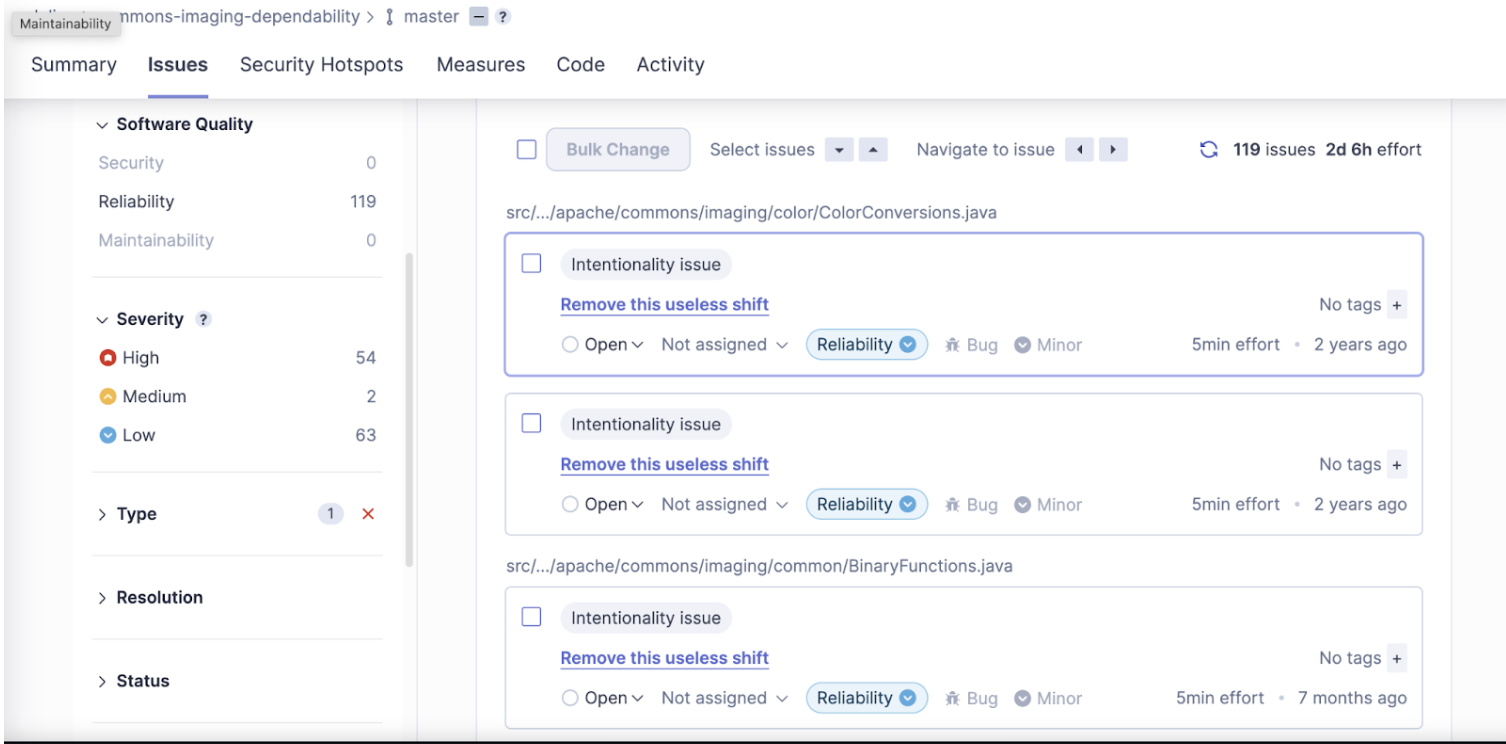
\includegraphics[width=1\linewidth]{reportSonarCloud.png}
    \caption{Report before fix}
    \label{fig:enter-label}
\end{figure}


\subsection{Analyzing SonarCloud}

After analyzing the commons-imaging-dependability project on SonarCloud, we found the following issues in the code:

\textbf{High → 109}

In the high category, several errors are related to divisions where the divisor is not checked for the possibility of being 0. Therefore, if the divisor is 0, the code would throw an exception. There are also errors of the type where referencing a static member of a subclass from its parent during class initialization makes the code more fragile and prone to future errors. The program's execution will largely depend on the order of class and static member initialization.

\textbf{Medium → 2}

In the medium category, there are only 2 errors where an attempt is made to get the length of a palette that could be null.

\textbf{Low → 63}

Out of these 63 errors, most are related to the suggestion to remove a left shift, explaining that an int is a 32-bit variable and specifying that shifting an int by 32 is the same as shifting by 0, and shifting by 33 is the same as shifting by 1. Additionally, there are some errors related to number casting.

\subsection{Bugs Fixed}

To organize our tasks based on the errors found in \textbf{SonarCloud}, we created tasks in \textbf{JIRA}, and each of them was assigned to the three members of the group. We attempted to address the majority of the 119 issues related to reliability, of which we were able to fix XX.

\begin{figure}[h!]
    \centering
    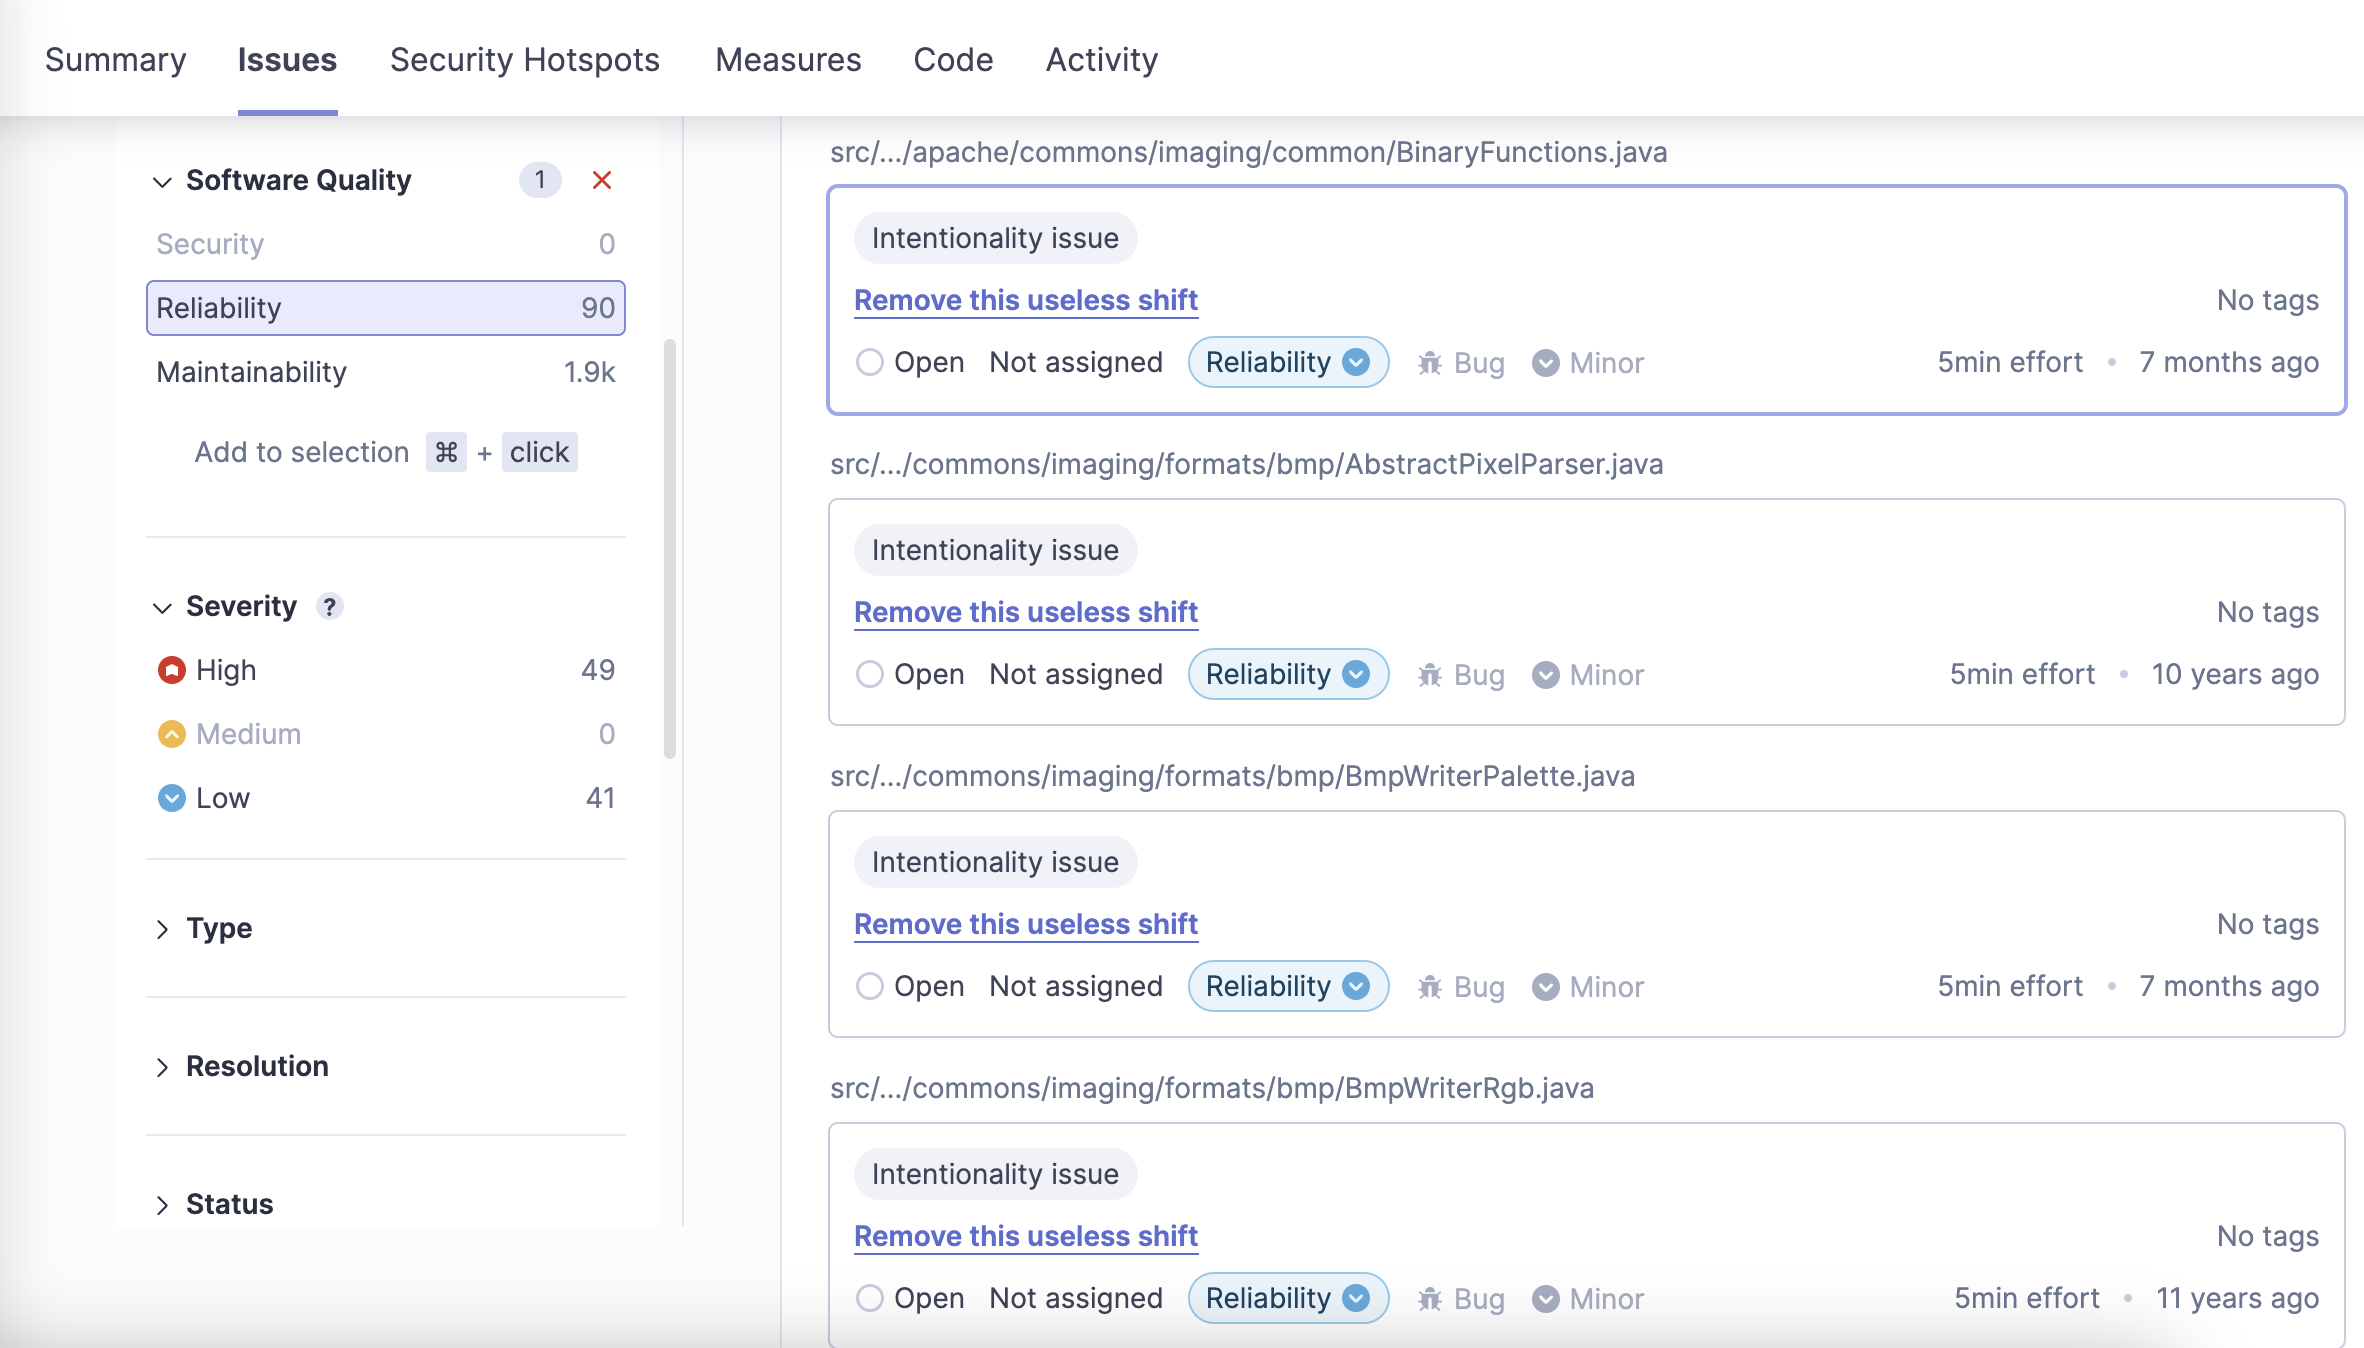
\includegraphics[width=1\linewidth]{reportSonarCloudFixed.png}
    \caption{Bugs Fixed}
    \label{fig:enter-label}
\end{figure}


\section{Software Testing Tools}

To measure and improve the robustness of the Apache Commons Imaging project's dependability, this section focuses on three key testing tools. First, we delve into the realm of code coverage using JaCoCo and CodeCov, unraveling their importance and impact. Following that, we explore mutation testing with PiTest, evaluating the resilience of test cases. The journey concludes with Java Microbenchmark Harness, providing insights into performance characteristics. Together, these tools form a robust arsenal to fortify and enhance the project's reliability.

\subsection{Code Coverage - JaCoCo}
JaCoCo \cite{jacoco} (Java Code Coverage) serves as a vital tool in assessing code coverage for Java applications, offering valuable insights into the extent of code execution during testing. It generates comprehensive reports that pinpoint the specific portions of the code exercised by tests.

Our investigation utilizing JaCoCo revealed a baseline of 77\% Instructions Coverage and 63\% Branches Coverage. This includes specific metrics such as 2448/6213 missed cyclomatic complexities, 3931/17299 missed lines, 511/2539 missed methods, and 16/431 missed classes.

A notable feature of JaCoCo lies in its ability to set a minimum expected coverage. This proactive measure ensures that code changes maintain a predefined level of coverage \cite{jacoco-check-mojo}, contributing significantly to the overall robustness of the project.

\subsection{Code Coverage - CodeCov}
CodeCov \cite{codecov} emerges as an instrumental tool, orchestrating a meticulous examination of code coverage within the Apache Commons Imaging project. This sophisticated platform specializes in unraveling the intricacies of test suite effectiveness.

\textbf{Key Metrics:}
\begin{enumerate}
    \item \textbf{Overall Code Coverage:} Our CodeCov analysis reveals a comprehensive code coverage of 71.17\% across the entirety of the project. This quantitative metric serves as a substantive indicator of the extent to which our test suites engage with the codebase.
    
    \item \textbf{Files with Lower Coverage Rates (In use with Below 0\%):}
    \begin{itemize}
        \item \texttt ColorTools.java
        \item \texttt PixelDensity.java
        \item \texttt DataParserBitmap.java
        \item \texttt TagInfoSLongs.java
        \item \texttt ColorTools.java
        \item \texttt PbmWriter.java
        \item \texttt PgmWriter.java
        \item \texttt UncompressedDataReader.java
        \item \texttt ScanExpediterInterlaced.java
        \item \texttt PhotometricInterpreterCieLab.java
        \item \texttt PhotometricInterpreterYCbCr.java
        \item \texttt FieldTypeFloat.java
    \end{itemize}
    
    \item \textbf{Line Coverage:} A granular examination exposes that among the 17,299 lines constituting the project, the project covers 12,311 lines.
\end{enumerate}

Following the addition of targeted tests aimed at addressing files with 0\% coverage, the overall code coverage has substantially increased to 71.82\%. Out of a total of 17,303 lines, 12,427 are now covered. Notably, certain sections of the code remain only partially covered, emphasizing the ongoing commitment to fortify the software's robustness and reliability.


\subsection{Mutation Testing - PiTest}
TODO

\subsection{Java Microbenchmark Harness}
JMH\cite{jmh} is a powerful tool specifically designed for benchmarking Java code, allowing us to meticulously analyze the performance of our compression algorithms.

In the context of our image management project, an in-depth analysis of CPU-intensive image formats has revealed TIFF and WebP as the most demanding formats in terms of system resources. Following this, a detailed examination of test durations highlighted a specific, time-consuming scenario (\texttt{org.apache.commons.\\imaging.formats.tiff.TiffRoundtripTest.test}): the compression of TIFF images utilizing various algorithms (\texttt{TIFF\_COMPRESSION\_\\LZW}, \texttt{TIFF\_COMPRESSION\_PACKBITS}, \texttt{TIFF\_COMPRESSION\_DEFLATE\_\\ADOBE}, and \texttt{Uncompressed}).


To further explore the performance of each compression algorithm applied separately to the same set of images, we conducted a benchmark, yielding the following results: \vspace{12pt}

\textbf{Before Parallelization:}
\begin{itemize}
    \item \texttt{TIFF\_COMPRESSION\_DEFLATE\_ADOBE:} Throughput 0.465 $\pm$ 0.006 ops/s
    \item \texttt{TIFF\_COMPRESSION\_LZW:} Throughput 0.216 $\pm$ 0.001 ops/s
    \item \texttt{TIFF\_COMPRESSION\_PACKBITS:} Throughput 1.278 $\pm$ 0.053 ops/s
    \item \texttt{Uncompressed:} Throughput 2.170 $\pm$ 0.019 ops/s
\end{itemize}

Upon thorough review, we identified an opportunity for performance enhancement by introducing parallelism into the compression process. The parallel application of compression algorithms resulted in significant throughput improvements:\vspace{12pt}

\textbf{After Parallelization:}
\begin{itemize}
    \item \texttt{TIFF\_COMPRESSION\_DEFLATE\_ADOBE:} Throughput 1.375 $\pm$ 0.012 ops/s (Increase by 196.77\%)
    \item \texttt{TIFF\_COMPRESSION\_LZW:} Throughput 0.774 $\pm$ 0.008 ops/s (Increase by 258.33\%)
    \item \texttt{TIFF\_COMPRESSION\_PACKBITS:} Throughput 2.870 $\pm$ 0.164 ops/s (Increase by 124.61\%)
    \item \texttt{Uncompressed:} Throughput 3.984 $\pm$ 0.066 ops/s (Increase by 83.12\%)
\end{itemize}

Beyond benchmark results, we observed a substantial reduction in the tiff test duration, decreasing from 8.4978 $\pm$ 0.0407 seconds ($\pm$0.48\%) to 3.7254 $\pm$ 0.128 seconds ($\pm$3.44\%) with the implemented parallelization. This notable improvement not only enhances the efficiency of our compression algorithms but also contributes to a more expedited execution of test scenarios.


\section{Automated Generation of Test Cases}
TODO

\subsection{EvoSuite}
TODO

\subsection{Randoop}
TODO

\section{Software Vulnerabilities}
TODO

\subsection{OWASP Dependability Checker}
TODO

\subsection{FindSecBugs (SpotBug)}
TODO

\section{Discussion}
TODO

\section{Conclusion}
TODO

%%
%% The acknowledgments section is defined using the "acks" environment
%% (and NOT an unnumbered section). This ensures the proper
%% identification of the section in the article metadata, and the
%% consistent spelling of the heading.
\begin{acks}
To the group, for always bringing "mate" while working.
\end{acks}

%% -> REFERENCES Section --> sample-base.bib has the cite references descriptions.
%% The next two lines define the bibliography style to be used, and
%% the bibliography file.

\bibliographystyle{ACM-Reference-Format}
\bibliography{sample-base}

%%
%% If your work has an appendix, this is the place to put it.
\appendix

\section{Research Methods}

\subsection{Part One}
TODO

\section{Online Resources}
TODO

\end{document}